\documentclass[1p]{elsarticle_modified}
%\bibliographystyle{elsarticle-num}

%\usepackage[colorlinks]{hyperref}
%\usepackage{abbrmath_seonhwa} %\Abb, \Ascr, \Acal ,\Abf, \Afrak
\usepackage{amsfonts}
\usepackage{amssymb}
\usepackage{amsmath}
\usepackage{amsthm}
\usepackage{scalefnt}
\usepackage{amsbsy}
\usepackage{kotex}
\usepackage{caption}
\usepackage{subfig}
\usepackage{color}
\usepackage{graphicx}
\usepackage{xcolor} %% white, black, red, green, blue, cyan, magenta, yellow
\usepackage{float}
\usepackage{setspace}
\usepackage{hyperref}

\usepackage{tikz}
\usetikzlibrary{arrows}

\usepackage{multirow}
\usepackage{array} % fixed length table
\usepackage{hhline}

%%%%%%%%%%%%%%%%%%%%%
\makeatletter
\renewcommand*\env@matrix[1][\arraystretch]{%
	\edef\arraystretch{#1}%
	\hskip -\arraycolsep
	\let\@ifnextchar\new@ifnextchar
	\array{*\c@MaxMatrixCols c}}
\makeatother %https://tex.stackexchange.com/questions/14071/how-can-i-increase-the-line-spacing-in-a-matrix
%%%%%%%%%%%%%%%

\usepackage[normalem]{ulem}

\newcommand{\msout}[1]{\ifmmode\text{\sout{\ensuremath{#1}}}\else\sout{#1}\fi}
%SOURCE: \msout is \stkout macro in https://tex.stackexchange.com/questions/20609/strikeout-in-math-mode

\newcommand{\cancel}[1]{
	\ifmmode
	{\color{red}\msout{#1}}
	\else
	{\color{red}\sout{#1}}
	\fi
}

\newcommand{\add}[1]{
	{\color{blue}\uwave{#1}}
}

\newcommand{\replace}[2]{
	\ifmmode
	{\color{red}\msout{#1}}{\color{blue}\uwave{#2}}
	\else
	{\color{red}\sout{#1}}{\color{blue}\uwave{#2}}
	\fi
}

\newcommand{\Sol}{\mathcal{S}} %segment
\newcommand{\D}{D} %diagram
\newcommand{\A}{\mathcal{A}} %arc


%%%%%%%%%%%%%%%%%%%%%%%%%%%%%5 test

\def\sl{\operatorname{\textup{SL}}(2,\Cbb)}
\def\psl{\operatorname{\textup{PSL}}(2,\Cbb)}
\def\quan{\mkern 1mu \triangleright \mkern 1mu}

\theoremstyle{definition}
\newtheorem{thm}{Theorem}[section]
\newtheorem{prop}[thm]{Proposition}
\newtheorem{lem}[thm]{Lemma}
\newtheorem{ques}[thm]{Question}
\newtheorem{cor}[thm]{Corollary}
\newtheorem{defn}[thm]{Definition}
\newtheorem{exam}[thm]{Example}
\newtheorem{rmk}[thm]{Remark}
\newtheorem{alg}[thm]{Algorithm}

\newcommand{\I}{\sqrt{-1}}
\begin{document}

%\begin{frontmatter}
%
%\title{Boundary parabolic representations of knots up to 8 crossings}
%
%%% Group authors per affiliation:
%\author{Yunhi Cho} 
%\address{Department of Mathematics, University of Seoul, Seoul, Korea}
%\ead{yhcho@uos.ac.kr}
%
%
%\author{Seonhwa Kim} %\fnref{s_kim}}
%\address{Center for Geometry and Physics, Institute for Basic Science, Pohang, 37673, Korea}
%\ead{ryeona17@ibs.re.kr}
%
%\author{Hyuk Kim}
%\address{Department of Mathematical Sciences, Seoul National University, Seoul 08826, Korea}
%\ead{hyukkim@snu.ac.kr}
%
%\author{Seokbeom Yoon}
%\address{Department of Mathematical Sciences, Seoul National University, Seoul, 08826,  Korea}
%\ead{sbyoon15@snu.ac.kr}
%
%\begin{abstract}
%We find all boundary parabolic representation of knots up to 8 crossings.
%
%\end{abstract}
%\begin{keyword}
%    \MSC[2010] 57M25 
%\end{keyword}
%
%\end{frontmatter}

%\linenumbers
%\tableofcontents
%
\newcommand\colored[1]{\textcolor{white}{\rule[-0.35ex]{0.8em}{1.4ex}}\kern-0.8em\color{red} #1}%
%\newcommand\colored[1]{\textcolor{white}{ #1}\kern-2.17ex	\textcolor{white}{ #1}\kern-1.81ex	\textcolor{white}{ #1}\kern-2.15ex\color{red}#1	}

{\Large $\underline{12a_{0285}~(K12a_{0285})}$}

\setlength{\tabcolsep}{10pt}
\renewcommand{\arraystretch}{1.6}
\vspace{1cm}\begin{tabular}{m{100pt}>{\centering\arraybackslash}m{274pt}}
\multirow{5}{120pt}{
	\centering
	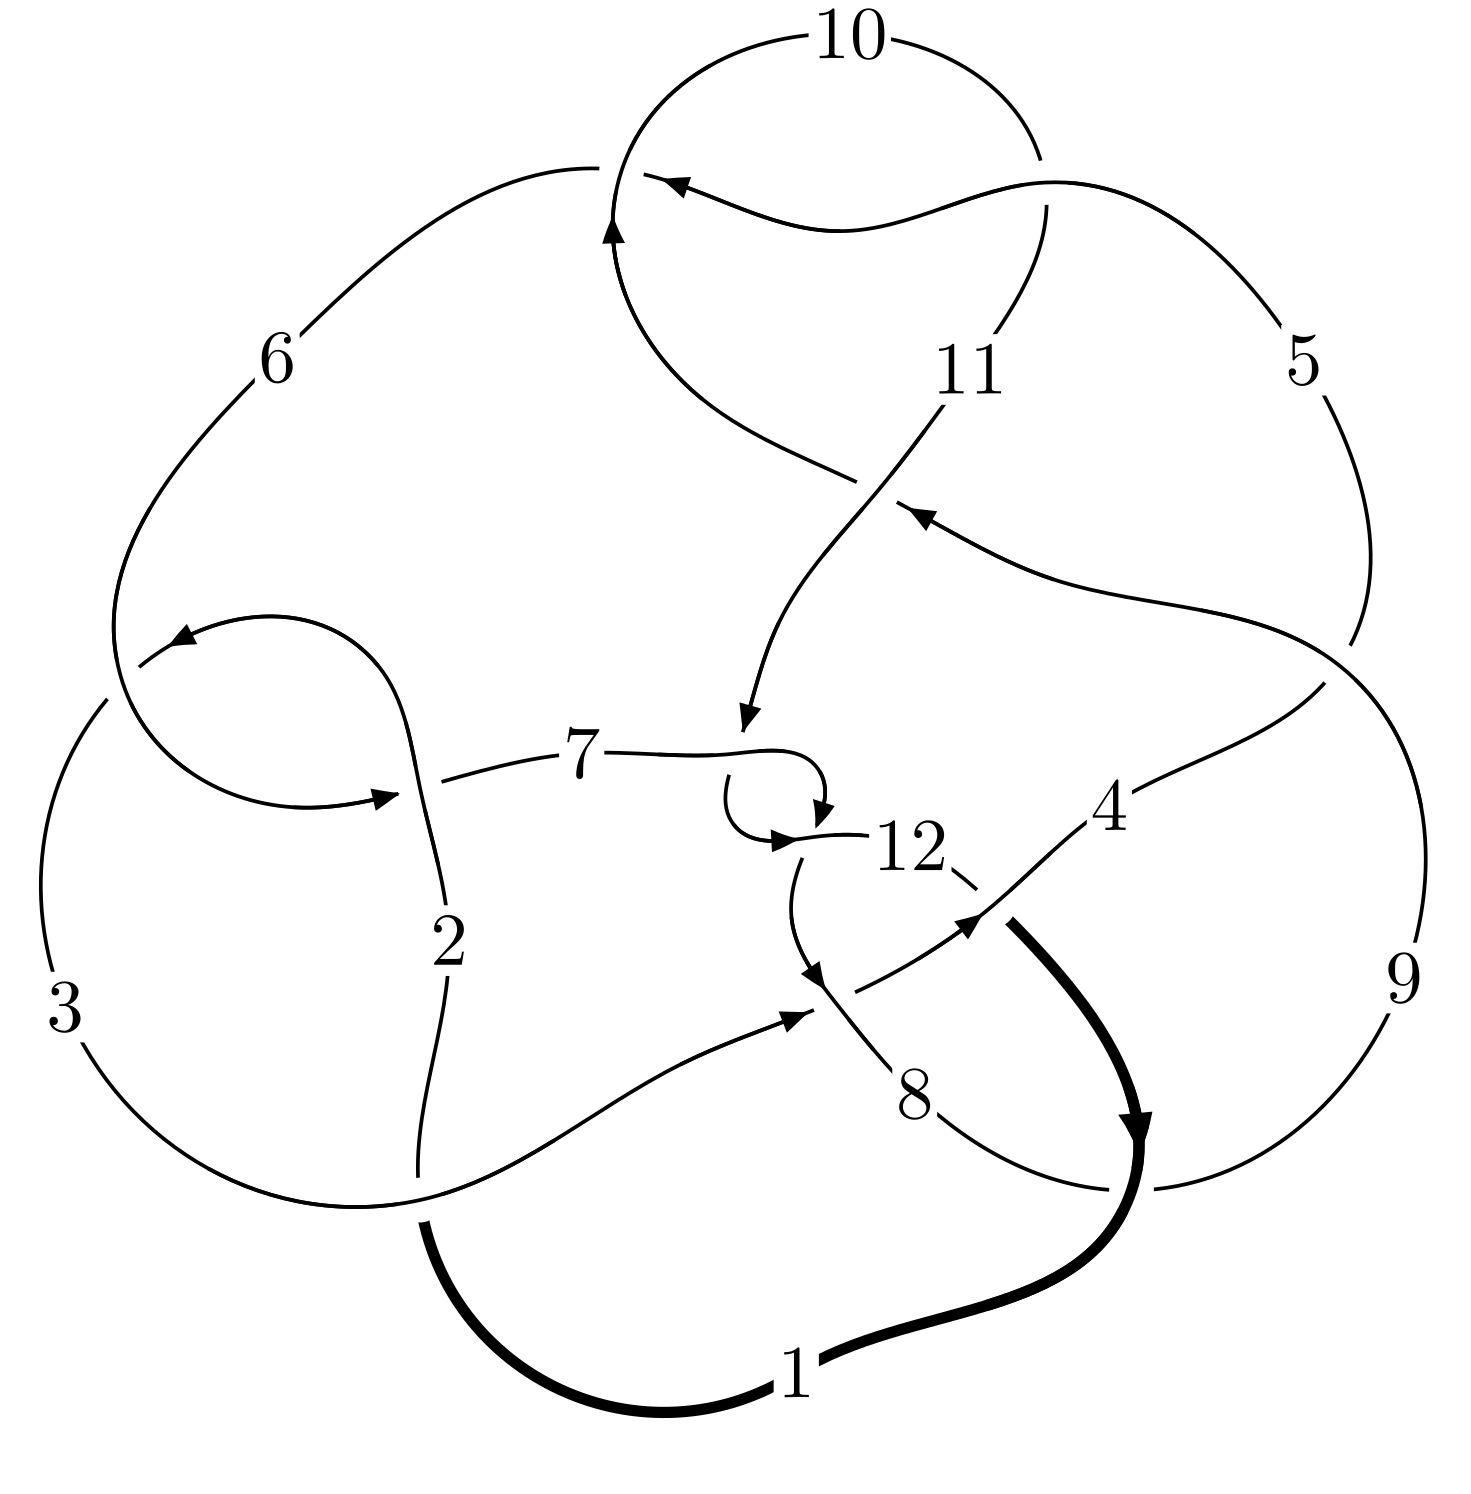
\includegraphics[width=112pt]{../../../GIT/diagram.site/Diagrams/png/1086_12a_0285.png}\\
\ \ \ A knot diagram\footnotemark}&
\allowdisplaybreaks
\textbf{Linearized knot diagam} \\
\cline{2-2}
 &
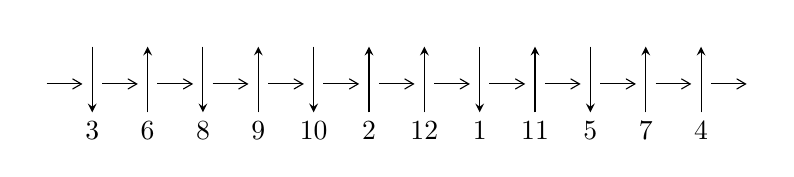
\begin{tikzpicture}[x=20pt, y=17pt]
	% nodes
	\node (C0) at (0, 0) {};
	\node (C1) at (1, 0) {};
	\node (C1U) at (1, +1) {};
	\node (C1D) at (1, -1) {3};

	\node (C2) at (2, 0) {};
	\node (C2U) at (2, +1) {};
	\node (C2D) at (2, -1) {6};

	\node (C3) at (3, 0) {};
	\node (C3U) at (3, +1) {};
	\node (C3D) at (3, -1) {8};

	\node (C4) at (4, 0) {};
	\node (C4U) at (4, +1) {};
	\node (C4D) at (4, -1) {9};

	\node (C5) at (5, 0) {};
	\node (C5U) at (5, +1) {};
	\node (C5D) at (5, -1) {10};

	\node (C6) at (6, 0) {};
	\node (C6U) at (6, +1) {};
	\node (C6D) at (6, -1) {2};

	\node (C7) at (7, 0) {};
	\node (C7U) at (7, +1) {};
	\node (C7D) at (7, -1) {12};

	\node (C8) at (8, 0) {};
	\node (C8U) at (8, +1) {};
	\node (C8D) at (8, -1) {1};

	\node (C9) at (9, 0) {};
	\node (C9U) at (9, +1) {};
	\node (C9D) at (9, -1) {11};

	\node (C10) at (10, 0) {};
	\node (C10U) at (10, +1) {};
	\node (C10D) at (10, -1) {5};

	\node (C11) at (11, 0) {};
	\node (C11U) at (11, +1) {};
	\node (C11D) at (11, -1) {7};

	\node (C12) at (12, 0) {};
	\node (C12U) at (12, +1) {};
	\node (C12D) at (12, -1) {4};
	\node (C13) at (13, 0) {};

	% arrows
	\draw[->,>={angle 60}]
	(C0) edge (C1) (C1) edge (C2) (C2) edge (C3) (C3) edge (C4) (C4) edge (C5) (C5) edge (C6) (C6) edge (C7) (C7) edge (C8) (C8) edge (C9) (C9) edge (C10) (C10) edge (C11) (C11) edge (C12) (C12) edge (C13) ;	\draw[->,>=stealth]
	(C1U) edge (C1D) (C2D) edge (C2U) (C3U) edge (C3D) (C4D) edge (C4U) (C5U) edge (C5D) (C6D) edge (C6U) (C7D) edge (C7U) (C8U) edge (C8D) (C9D) edge (C9U) (C10U) edge (C10D) (C11D) edge (C11U) (C12D) edge (C12U) ;
	\end{tikzpicture} \\
\hhline{~~} \\& 
\textbf{Solving Sequence} \\ \cline{2-2} 
 &
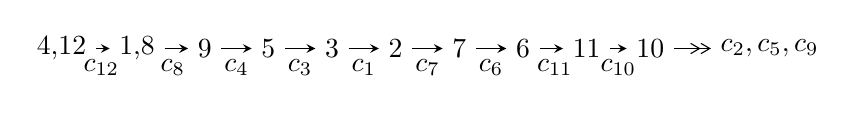
\begin{tikzpicture}[x=23pt, y=7pt]
	% node
	\node (A0) at (-1/8, 0) {4,12};
	\node (A1) at (17/16, 0) {1,8};
	\node (A2) at (17/8, 0) {9};
	\node (A3) at (25/8, 0) {5};
	\node (A4) at (33/8, 0) {3};
	\node (A5) at (41/8, 0) {2};
	\node (A6) at (49/8, 0) {7};
	\node (A7) at (57/8, 0) {6};
	\node (A8) at (65/8, 0) {11};
	\node (A9) at (73/8, 0) {10};
	\node (C1) at (1/2, -1) {$c_{12}$};
	\node (C2) at (13/8, -1) {$c_{8}$};
	\node (C3) at (21/8, -1) {$c_{4}$};
	\node (C4) at (29/8, -1) {$c_{3}$};
	\node (C5) at (37/8, -1) {$c_{1}$};
	\node (C6) at (45/8, -1) {$c_{7}$};
	\node (C7) at (53/8, -1) {$c_{6}$};
	\node (C8) at (61/8, -1) {$c_{11}$};
	\node (C9) at (69/8, -1) {$c_{10}$};
	\node (A10) at (11, 0) {$c_{2},c_{5},c_{9}$};

	% edge
	\draw[->,>=stealth]	
	(A0) edge (A1) (A1) edge (A2) (A2) edge (A3) (A3) edge (A4) (A4) edge (A5) (A5) edge (A6) (A6) edge (A7) (A7) edge (A8) (A8) edge (A9) ;
	\draw[->>,>={angle 60}]	
	(A9) edge (A10);
\end{tikzpicture} \\ 

\end{tabular} \\

\footnotetext{
The image of knot diagram is generated by the software ``\textbf{Draw programme}" developed by Andrew Bartholomew(\url{http://www.layer8.co.uk/maths/draw/index.htm\#Running-draw}), where we modified some parts for our purpose(\url{https://github.com/CATsTAILs/LinksPainter}).
}\phantom \\ \newline 
\centering \textbf{Ideals for irreducible components\footnotemark of $X_{\text{par}}$} 
 
\begin{align*}
I^u_{1}&=\langle 
-4.38602\times10^{1011} u^{142}+4.52733\times10^{1012} u^{141}+\cdots+7.36925\times10^{1008} b-6.46995\times10^{1015},\\
\phantom{I^u_{1}}&\phantom{= \langle  }5.01535\times10^{1015} u^{142}-5.18424\times10^{1016} u^{141}+\cdots+7.49969\times10^{1012} a+7.61449\times10^{1019},\\
\phantom{I^u_{1}}&\phantom{= \langle  }u^{143}-11 u^{142}+\cdots+27584 u-10177\rangle \\
I^u_{2}&=\langle 
17434253328675 u^{29}-10533896428578 u^{28}+\cdots+320682258343 b+24639564912626,\\
\phantom{I^u_{2}}&\phantom{= \langle  }-14129515908963 u^{29}+10877469922460 u^{28}+\cdots+320682258343 a-14905932574354,\\
\phantom{I^u_{2}}&\phantom{= \langle  }u^{30}-4 u^{28}+\cdots+7 u+1\rangle \\
\\
\end{align*}
\raggedright * 2 irreducible components of $\dim_{\mathbb{C}}=0$, with total 173 representations.\\
\footnotetext{All coefficients of polynomials are rational numbers. But the coefficients are sometimes approximated in decimal forms when there is not enough margin.}
\newpage
\renewcommand{\arraystretch}{1}
\centering \section*{I. $I^u_{1}= \langle -4.39\times10^{1011} u^{142}+4.53\times10^{1012} u^{141}+\cdots+7.37\times10^{1008} b-6.47\times10^{1015},\;5.02\times10^{1015} u^{142}-5.18\times10^{1016} u^{141}+\cdots+7.50\times10^{1012} a+7.61\times10^{1019},\;u^{143}-11 u^{142}+\cdots+27584 u-10177 \rangle$}
\flushleft \textbf{(i) Arc colorings}\\
\begin{tabular}{m{7pt} m{180pt} m{7pt} m{180pt} }
\flushright $a_{4}=$&$\begin{pmatrix}0\\u\end{pmatrix}$ \\
\flushright $a_{12}=$&$\begin{pmatrix}1\\0\end{pmatrix}$ \\
\flushright $a_{1}=$&$\begin{pmatrix}1\\- u^2\end{pmatrix}$ \\
\flushright $a_{8}=$&$\begin{pmatrix}-668.741 u^{142}+6912.61 u^{141}+\cdots+1.21975\times10^{7} u-1.01531\times10^{7}\\595.179 u^{142}-6143.54 u^{141}+\cdots-1.08740\times10^{7} u+8.77965\times10^{6}\end{pmatrix}$ \\
\flushright $a_{9}=$&$\begin{pmatrix}-967.389 u^{142}+9991.06 u^{141}+\cdots+1.76427\times10^{7} u-1.44188\times10^{7}\\740.258 u^{142}-7639.69 u^{141}+\cdots-1.35358\times10^{7} u+1.08831\times10^{7}\end{pmatrix}$ \\
\flushright $a_{5}=$&$\begin{pmatrix}-108.766 u^{142}+1139.76 u^{141}+\cdots+1.37302\times10^{6} u-1.61760\times10^{6}\\18.0614 u^{142}-178.616 u^{141}+\cdots-432383. u+112725.\end{pmatrix}$ \\
\flushright $a_{3}=$&$\begin{pmatrix}259.463 u^{142}-2660.28 u^{141}+\cdots-5.64469\times10^{6} u+4.01611\times10^{6}\\259.478 u^{142}-2699.21 u^{141}+\cdots-4.33611\times10^{6} u+4.12531\times10^{6}\end{pmatrix}$ \\
\flushright $a_{2}=$&$\begin{pmatrix}-211.226 u^{142}+2185.46 u^{141}+\cdots+3.35948\times10^{6} u-2.87681\times10^{6}\\386.427 u^{142}-3993.28 u^{141}+\cdots-6.92165\times10^{6} u+5.73513\times10^{6}\end{pmatrix}$ \\
\flushright $a_{7}=$&$\begin{pmatrix}-1263.92 u^{142}+13056.2 u^{141}+\cdots+2.30715\times10^{7} u-1.89327\times10^{7}\\595.179 u^{142}-6143.54 u^{141}+\cdots-1.08740\times10^{7} u+8.77965\times10^{6}\end{pmatrix}$ \\
\flushright $a_{6}=$&$\begin{pmatrix}-619.595 u^{142}+6371.78 u^{141}+\cdots+1.24532\times10^{7} u-9.34184\times10^{6}\\-226.209 u^{142}+2361.85 u^{141}+\cdots+3.61819\times10^{6} u-3.74097\times10^{6}\end{pmatrix}$ \\
\flushright $a_{11}=$&$\begin{pmatrix}164.959 u^{142}-1704.00 u^{141}+\cdots-3.34405\times10^{6} u+2.71769\times10^{6}\\240.397 u^{142}-2495.44 u^{141}+\cdots-4.61159\times10^{6} u+4.12755\times10^{6}\end{pmatrix}$ \\
\flushright $a_{10}=$&$\begin{pmatrix}1277.48 u^{142}-13220.8 u^{141}+\cdots-2.34740\times10^{7} u+1.99571\times10^{7}\\-1249.41 u^{142}+12921.3 u^{141}+\cdots+2.29038\times10^{7} u-1.92225\times10^{7}\end{pmatrix}$\\&\end{tabular}
\flushleft \textbf{(ii) Obstruction class $= -1$}\\~\\
\flushleft \textbf{(iii) Cusp Shapes $= -2985.35 u^{142}+30817.6 u^{141}+\cdots+5.50221\times10^{7} u-4.46363\times10^{7}$}\\~\\
\newpage\renewcommand{\arraystretch}{1}
\flushleft \textbf{(iv) u-Polynomials at the component}\newline \\
\begin{tabular}{m{50pt}|m{274pt}}
Crossings & \hspace{64pt}u-Polynomials at each crossing \\
\hline $$\begin{aligned}c_{1}\end{aligned}$$&$\begin{aligned}
&u^{143}+54 u^{142}+\cdots-64 u-1
\end{aligned}$\\
\hline $$\begin{aligned}c_{2},c_{6}\end{aligned}$$&$\begin{aligned}
&u^{143}+27 u^{141}+\cdots+14 u-1
\end{aligned}$\\
\hline $$\begin{aligned}c_{3}\end{aligned}$$&$\begin{aligned}
&u^{143}- u^{142}+\cdots-79259 u-20259
\end{aligned}$\\
\hline $$\begin{aligned}c_{4}\end{aligned}$$&$\begin{aligned}
&u^{143}+u^{142}+\cdots+7060687 u-934895
\end{aligned}$\\
\hline $$\begin{aligned}c_{5},c_{10}\end{aligned}$$&$\begin{aligned}
&u^{143}- u^{142}+\cdots+11 u-19
\end{aligned}$\\
\hline $$\begin{aligned}c_{7},c_{11}\end{aligned}$$&$\begin{aligned}
&u^{143}+u^{142}+\cdots+4691957 u-772753
\end{aligned}$\\
\hline $$\begin{aligned}c_{8}\end{aligned}$$&$\begin{aligned}
&u^{143}+5 u^{142}+\cdots-58437 u-10229
\end{aligned}$\\
\hline $$\begin{aligned}c_{9}\end{aligned}$$&$\begin{aligned}
&u^{143}-75 u^{142}+\cdots-6035 u+361
\end{aligned}$\\
\hline $$\begin{aligned}c_{12}\end{aligned}$$&$\begin{aligned}
&u^{143}+11 u^{142}+\cdots+27584 u+10177
\end{aligned}$\\
\hline
\end{tabular}\\~\\
\newpage\renewcommand{\arraystretch}{1}
\flushleft \textbf{(v) Riley Polynomials at the component}\newline \\
\begin{tabular}{m{50pt}|m{274pt}}
Crossings & \hspace{64pt}Riley Polynomials at each crossing \\
\hline $$\begin{aligned}c_{1}\end{aligned}$$&$\begin{aligned}
&y^{143}+86 y^{142}+\cdots+12060 y-1
\end{aligned}$\\
\hline $$\begin{aligned}c_{2},c_{6}\end{aligned}$$&$\begin{aligned}
&y^{143}+54 y^{142}+\cdots-64 y-1
\end{aligned}$\\
\hline $$\begin{aligned}c_{3}\end{aligned}$$&$\begin{aligned}
&y^{143}+35 y^{142}+\cdots-29282604383 y-410427081
\end{aligned}$\\
\hline $$\begin{aligned}c_{4}\end{aligned}$$&$\begin{aligned}
&y^{143}-93 y^{142}+\cdots-27555367489641 y-874028661025
\end{aligned}$\\
\hline $$\begin{aligned}c_{5},c_{10}\end{aligned}$$&$\begin{aligned}
&y^{143}+75 y^{142}+\cdots-6035 y-361
\end{aligned}$\\
\hline $$\begin{aligned}c_{7},c_{11}\end{aligned}$$&$\begin{aligned}
&y^{143}-117 y^{142}+\cdots-6329951089997 y-597147199009
\end{aligned}$\\
\hline $$\begin{aligned}c_{8}\end{aligned}$$&$\begin{aligned}
&y^{143}+33 y^{142}+\cdots-8154279695 y-104632441
\end{aligned}$\\
\hline $$\begin{aligned}c_{9}\end{aligned}$$&$\begin{aligned}
&y^{143}-9 y^{142}+\cdots+5558613 y-130321
\end{aligned}$\\
\hline $$\begin{aligned}c_{12}\end{aligned}$$&$\begin{aligned}
&y^{143}-37 y^{142}+\cdots+2435807716 y-103571329
\end{aligned}$\\
\hline
\end{tabular}\\~\\
\newpage\flushleft \textbf{(vi) Complex Volumes and Cusp Shapes}
$$\begin{array}{c|c|c}  
\text{Solutions to }I^u_{1}& \I (\text{vol} + \sqrt{-1}CS) & \text{Cusp shape}\\
 \hline 
\begin{aligned}
u &= -0.942702 + 0.364107 I \\
a &= -0.177763 - 1.145760 I \\
b &= \phantom{-}0.866397 - 0.753553 I\end{aligned}
 & \phantom{-}1.72885 - 1.29757 I & \phantom{-0.000000 } 0 \\ \hline\begin{aligned}
u &= -0.942702 - 0.364107 I \\
a &= -0.177763 + 1.145760 I \\
b &= \phantom{-}0.866397 + 0.753553 I\end{aligned}
 & \phantom{-}1.72885 + 1.29757 I & \phantom{-0.000000 } 0 \\ \hline\begin{aligned}
u &= -0.686690 + 0.770176 I \\
a &= \phantom{-}0.80784 - 1.60288 I \\
b &= \phantom{-}1.116190 - 0.098548 I\end{aligned}
 & \phantom{-}1.45725 - 0.56929 I & \phantom{-0.000000 } 0 \\ \hline\begin{aligned}
u &= -0.686690 - 0.770176 I \\
a &= \phantom{-}0.80784 + 1.60288 I \\
b &= \phantom{-}1.116190 + 0.098548 I\end{aligned}
 & \phantom{-}1.45725 + 0.56929 I & \phantom{-0.000000 } 0 \\ \hline\begin{aligned}
u &= -0.672172 + 0.673426 I \\
a &= \phantom{-}1.126840 - 0.440477 I \\
b &= \phantom{-}0.282383 + 0.300551 I\end{aligned}
 & \phantom{-}1.20400 - 2.16328 I & \phantom{-0.000000 } 0 \\ \hline\begin{aligned}
u &= -0.672172 - 0.673426 I \\
a &= \phantom{-}1.126840 + 0.440477 I \\
b &= \phantom{-}0.282383 - 0.300551 I\end{aligned}
 & \phantom{-}1.20400 + 2.16328 I & \phantom{-0.000000 } 0 \\ \hline\begin{aligned}
u &= -0.790822 + 0.688856 I \\
a &= \phantom{-}0.102784 - 1.035030 I \\
b &= \phantom{-}0.348736 - 1.110730 I\end{aligned}
 & \phantom{-}1.33673 - 2.51070 I & \phantom{-0.000000 } 0 \\ \hline\begin{aligned}
u &= -0.790822 - 0.688856 I \\
a &= \phantom{-}0.102784 + 1.035030 I \\
b &= \phantom{-}0.348736 + 1.110730 I\end{aligned}
 & \phantom{-}1.33673 + 2.51070 I & \phantom{-0.000000 } 0 \\ \hline\begin{aligned}
u &= \phantom{-}0.698246 + 0.784390 I \\
a &= \phantom{-}0.52856 + 1.79612 I \\
b &= \phantom{-}1.224570 + 0.258360 I\end{aligned}
 & \phantom{-}0.75296 + 5.48494 I & \phantom{-0.000000 } 0 \\ \hline\begin{aligned}
u &= \phantom{-}0.698246 - 0.784390 I \\
a &= \phantom{-}0.52856 - 1.79612 I \\
b &= \phantom{-}1.224570 - 0.258360 I\end{aligned}
 & \phantom{-}0.75296 - 5.48494 I & \phantom{-0.000000 } 0\\
 \hline 
 \end{array}$$\newpage$$\begin{array}{c|c|c}  
\text{Solutions to }I^u_{1}& \I (\text{vol} + \sqrt{-1}CS) & \text{Cusp shape}\\
 \hline 
\begin{aligned}
u &= \phantom{-}0.412417 + 0.855264 I \\
a &= -0.058546 + 0.861634 I \\
b &= -0.394352 + 0.734852 I\end{aligned}
 & -4.53599 + 0.12727 I & \phantom{-0.000000 } 0 \\ \hline\begin{aligned}
u &= \phantom{-}0.412417 - 0.855264 I \\
a &= -0.058546 - 0.861634 I \\
b &= -0.394352 - 0.734852 I\end{aligned}
 & -4.53599 - 0.12727 I & \phantom{-0.000000 } 0 \\ \hline\begin{aligned}
u &= -0.619462 + 0.714333 I \\
a &= \phantom{-}0.504812 - 0.994420 I \\
b &= \phantom{-}0.640043 - 0.456237 I\end{aligned}
 & \phantom{-}0.41349 - 1.81846 I & \phantom{-0.000000 } 0 \\ \hline\begin{aligned}
u &= -0.619462 - 0.714333 I \\
a &= \phantom{-}0.504812 + 0.994420 I \\
b &= \phantom{-}0.640043 + 0.456237 I\end{aligned}
 & \phantom{-}0.41349 + 1.81846 I & \phantom{-0.000000 } 0 \\ \hline\begin{aligned}
u &= \phantom{-}0.746098 + 0.578824 I \\
a &= \phantom{-}1.144860 - 0.020941 I \\
b &= -0.072007 - 0.458537 I\end{aligned}
 & \phantom{-}0.43136 - 2.64878 I & \phantom{-0.000000 } 0 \\ \hline\begin{aligned}
u &= \phantom{-}0.746098 - 0.578824 I \\
a &= \phantom{-}1.144860 + 0.020941 I \\
b &= -0.072007 + 0.458537 I\end{aligned}
 & \phantom{-}0.43136 + 2.64878 I & \phantom{-0.000000 } 0 \\ \hline\begin{aligned}
u &= \phantom{-}0.956217 + 0.473910 I \\
a &= -0.459363 + 0.933946 I \\
b &= \phantom{-}0.835719 + 0.735845 I\end{aligned}
 & \phantom{-}1.57409 + 4.33045 I & \phantom{-0.000000 } 0 \\ \hline\begin{aligned}
u &= \phantom{-}0.956217 - 0.473910 I \\
a &= -0.459363 - 0.933946 I \\
b &= \phantom{-}0.835719 - 0.735845 I\end{aligned}
 & \phantom{-}1.57409 - 4.33045 I & \phantom{-0.000000 } 0 \\ \hline\begin{aligned}
u &= -0.907918 + 0.065941 I \\
a &= \phantom{-}0.599867 + 1.261830 I \\
b &= -1.162300 + 0.466689 I\end{aligned}
 & \phantom{-}4.14311 - 3.74371 I & \phantom{-0.000000 } 0 \\ \hline\begin{aligned}
u &= -0.907918 - 0.065941 I \\
a &= \phantom{-}0.599867 - 1.261830 I \\
b &= -1.162300 - 0.466689 I\end{aligned}
 & \phantom{-}4.14311 + 3.74371 I & \phantom{-0.000000 } 0\\
 \hline 
 \end{array}$$\newpage$$\begin{array}{c|c|c}  
\text{Solutions to }I^u_{1}& \I (\text{vol} + \sqrt{-1}CS) & \text{Cusp shape}\\
 \hline 
\begin{aligned}
u &= \phantom{-}0.778207 + 0.459641 I \\
a &= \phantom{-}0.155491 - 0.435491 I \\
b &= \phantom{-}0.300328 - 0.749291 I\end{aligned}
 & \phantom{-}0.710905 - 0.522185 I & \phantom{-0.000000 } 0 \\ \hline\begin{aligned}
u &= \phantom{-}0.778207 - 0.459641 I \\
a &= \phantom{-}0.155491 + 0.435491 I \\
b &= \phantom{-}0.300328 + 0.749291 I\end{aligned}
 & \phantom{-}0.710905 + 0.522185 I & \phantom{-0.000000 } 0 \\ \hline\begin{aligned}
u &= \phantom{-}0.824561 + 0.723923 I \\
a &= -0.052145 + 1.034410 I \\
b &= \phantom{-}0.120849 + 1.297670 I\end{aligned}
 & \phantom{-}0.27543 + 7.67403 I & \phantom{-0.000000 } 0 \\ \hline\begin{aligned}
u &= \phantom{-}0.824561 - 0.723923 I \\
a &= -0.052145 - 1.034410 I \\
b &= \phantom{-}0.120849 - 1.297670 I\end{aligned}
 & \phantom{-}0.27543 - 7.67403 I & \phantom{-0.000000 } 0 \\ \hline\begin{aligned}
u &= -0.866052 + 0.245513 I \\
a &= \phantom{-}0.92166 + 2.05840 I \\
b &= -1.291340 - 0.097348 I\end{aligned}
 & \phantom{-}9.48273 + 0.34349 I & \phantom{-0.000000 } 0 \\ \hline\begin{aligned}
u &= -0.866052 - 0.245513 I \\
a &= \phantom{-}0.92166 - 2.05840 I \\
b &= -1.291340 + 0.097348 I\end{aligned}
 & \phantom{-}9.48273 - 0.34349 I & \phantom{-0.000000 } 0 \\ \hline\begin{aligned}
u &= -0.998820 + 0.491964 I \\
a &= \phantom{-}0.254642 - 0.746212 I \\
b &= \phantom{-}1.189530 - 0.573878 I\end{aligned}
 & \phantom{-}2.83724 - 4.45710 I & \phantom{-0.000000 } 0 \\ \hline\begin{aligned}
u &= -0.998820 - 0.491964 I \\
a &= \phantom{-}0.254642 + 0.746212 I \\
b &= \phantom{-}1.189530 + 0.573878 I\end{aligned}
 & \phantom{-}2.83724 + 4.45710 I & \phantom{-0.000000 } 0 \\ \hline\begin{aligned}
u &= \phantom{-}0.692047 + 0.890082 I \\
a &= \phantom{-}0.029194 + 1.171020 I \\
b &= \phantom{-}0.989314 + 0.511122 I\end{aligned}
 & -2.05768 + 0.08833 I & \phantom{-0.000000 } 0 \\ \hline\begin{aligned}
u &= \phantom{-}0.692047 - 0.890082 I \\
a &= \phantom{-}0.029194 - 1.171020 I \\
b &= \phantom{-}0.989314 - 0.511122 I\end{aligned}
 & -2.05768 - 0.08833 I & \phantom{-0.000000 } 0\\
 \hline 
 \end{array}$$\newpage$$\begin{array}{c|c|c}  
\text{Solutions to }I^u_{1}& \I (\text{vol} + \sqrt{-1}CS) & \text{Cusp shape}\\
 \hline 
\begin{aligned}
u &= \phantom{-}0.764186 + 0.837668 I \\
a &= -0.041847 + 0.585377 I \\
b &= -0.302856 + 0.732268 I\end{aligned}
 & -3.47929 + 1.86853 I & \phantom{-0.000000 } 0 \\ \hline\begin{aligned}
u &= \phantom{-}0.764186 - 0.837668 I \\
a &= -0.041847 - 0.585377 I \\
b &= -0.302856 - 0.732268 I\end{aligned}
 & -3.47929 - 1.86853 I & \phantom{-0.000000 } 0 \\ \hline\begin{aligned}
u &= \phantom{-}0.831651 + 0.219641 I \\
a &= \phantom{-}1.35365 - 1.93595 I \\
b &= -1.398960 + 0.000957 I\end{aligned}
 & \phantom{-}9.76892 + 5.18382 I & \phantom{-0.000000 } 0 \\ \hline\begin{aligned}
u &= \phantom{-}0.831651 - 0.219641 I \\
a &= \phantom{-}1.35365 + 1.93595 I \\
b &= -1.398960 - 0.000957 I\end{aligned}
 & \phantom{-}9.76892 - 5.18382 I & \phantom{-0.000000 } 0 \\ \hline\begin{aligned}
u &= -0.856184 + 0.014229 I \\
a &= \phantom{-}0.050201 - 1.008980 I \\
b &= -1.56583 - 0.86229 I\end{aligned}
 & \phantom{-}7.41401 + 9.47262 I & \phantom{-0.000000 } 0 \\ \hline\begin{aligned}
u &= -0.856184 - 0.014229 I \\
a &= \phantom{-}0.050201 + 1.008980 I \\
b &= -1.56583 + 0.86229 I\end{aligned}
 & \phantom{-}7.41401 - 9.47262 I & \phantom{-0.000000 } 0 \\ \hline\begin{aligned}
u &= \phantom{-}0.728724 + 0.881909 I \\
a &= -0.906766 + 0.164729 I \\
b &= \phantom{-}0.050733 + 0.686342 I\end{aligned}
 & \phantom{-}3.53088 + 1.62729 I & \phantom{-0.000000 } 0 \\ \hline\begin{aligned}
u &= \phantom{-}0.728724 - 0.881909 I \\
a &= -0.906766 - 0.164729 I \\
b &= \phantom{-}0.050733 - 0.686342 I\end{aligned}
 & \phantom{-}3.53088 - 1.62729 I & \phantom{-0.000000 } 0 \\ \hline\begin{aligned}
u &= \phantom{-}0.923053 + 0.682792 I \\
a &= \phantom{-}0.137723 - 0.951706 I \\
b &= -0.336105 - 1.336030 I\end{aligned}
 & \phantom{-}4.25948 + 3.97292 I & \phantom{-0.000000 } 0 \\ \hline\begin{aligned}
u &= \phantom{-}0.923053 - 0.682792 I \\
a &= \phantom{-}0.137723 + 0.951706 I \\
b &= -0.336105 + 1.336030 I\end{aligned}
 & \phantom{-}4.25948 - 3.97292 I & \phantom{-0.000000 } 0\\
 \hline 
 \end{array}$$\newpage$$\begin{array}{c|c|c}  
\text{Solutions to }I^u_{1}& \I (\text{vol} + \sqrt{-1}CS) & \text{Cusp shape}\\
 \hline 
\begin{aligned}
u &= \phantom{-}0.228646 + 0.807230 I \\
a &= \phantom{-}0.023292 - 1.154560 I \\
b &= \phantom{-}0.484549 - 0.690336 I\end{aligned}
 & -3.54560 - 4.45890 I & \phantom{-0.000000 } 0 \\ \hline\begin{aligned}
u &= \phantom{-}0.228646 - 0.807230 I \\
a &= \phantom{-}0.023292 + 1.154560 I \\
b &= \phantom{-}0.484549 + 0.690336 I\end{aligned}
 & -3.54560 + 4.45890 I & \phantom{-0.000000 } 0 \\ \hline\begin{aligned}
u &= -0.824374 + 0.818767 I \\
a &= -0.134727 + 0.950498 I \\
b &= -0.330114 + 1.302230 I\end{aligned}
 & \phantom{-}4.19868 - 6.92087 I & \phantom{-0.000000 } 0 \\ \hline\begin{aligned}
u &= -0.824374 - 0.818767 I \\
a &= -0.134727 - 0.950498 I \\
b &= -0.330114 - 1.302230 I\end{aligned}
 & \phantom{-}4.19868 + 6.92087 I & \phantom{-0.000000 } 0 \\ \hline\begin{aligned}
u &= \phantom{-}0.850879 + 0.794220 I \\
a &= \phantom{-}0.002009 - 0.970973 I \\
b &= -0.09037 - 1.43673 I\end{aligned}
 & \phantom{-}3.18956 + 12.44830 I & \phantom{-0.000000 } 0 \\ \hline\begin{aligned}
u &= \phantom{-}0.850879 - 0.794220 I \\
a &= \phantom{-}0.002009 + 0.970973 I \\
b &= -0.09037 + 1.43673 I\end{aligned}
 & \phantom{-}3.18956 - 12.44830 I & \phantom{-0.000000 } 0 \\ \hline\begin{aligned}
u &= \phantom{-}0.825852 + 0.004693 I \\
a &= \phantom{-}0.095954 + 0.726046 I \\
b &= -1.71850 + 0.66219 I\end{aligned}
 & \phantom{-}8.39627 - 4.33805 I & \phantom{-0.000000 } 0 \\ \hline\begin{aligned}
u &= \phantom{-}0.825852 - 0.004693 I \\
a &= \phantom{-}0.095954 - 0.726046 I \\
b &= -1.71850 - 0.66219 I\end{aligned}
 & \phantom{-}8.39627 + 4.33805 I & \phantom{-0.000000 } 0 \\ \hline\begin{aligned}
u &= -0.967449 + 0.682030 I \\
a &= -0.009488 + 0.960374 I \\
b &= -0.597638 + 1.204970 I\end{aligned}
 & \phantom{-}4.75240 + 1.14948 I & \phantom{-0.000000 } 0 \\ \hline\begin{aligned}
u &= -0.967449 - 0.682030 I \\
a &= -0.009488 - 0.960374 I \\
b &= -0.597638 - 1.204970 I\end{aligned}
 & \phantom{-}4.75240 - 1.14948 I & \phantom{-0.000000 } 0\\
 \hline 
 \end{array}$$\newpage$$\begin{array}{c|c|c}  
\text{Solutions to }I^u_{1}& \I (\text{vol} + \sqrt{-1}CS) & \text{Cusp shape}\\
 \hline 
\begin{aligned}
u &= \phantom{-}0.572462 + 0.564106 I \\
a &= -0.02824 + 1.51493 I \\
b &= -0.175033 + 0.862926 I\end{aligned}
 & -2.32809 + 6.89844 I & \phantom{-0.000000 } 0 \\ \hline\begin{aligned}
u &= \phantom{-}0.572462 - 0.564106 I \\
a &= -0.02824 - 1.51493 I \\
b &= -0.175033 - 0.862926 I\end{aligned}
 & -2.32809 - 6.89844 I & \phantom{-0.000000 } 0 \\ \hline\begin{aligned}
u &= -1.081800 + 0.521766 I \\
a &= -0.667986 + 0.530010 I \\
b &= \phantom{-}0.050573 - 0.324471 I\end{aligned}
 & \phantom{-}5.22748 + 1.13720 I & \phantom{-0.000000 } 0 \\ \hline\begin{aligned}
u &= -1.081800 - 0.521766 I \\
a &= -0.667986 - 0.530010 I \\
b &= \phantom{-}0.050573 + 0.324471 I\end{aligned}
 & \phantom{-}5.22748 - 1.13720 I & \phantom{-0.000000 } 0 \\ \hline\begin{aligned}
u &= -0.784389 + 0.112607 I \\
a &= \phantom{-}0.099331 - 1.070910 I \\
b &= \phantom{-}1.52498 - 0.73193 I\end{aligned}
 & \phantom{-}4.58573 - 4.92230 I & \phantom{-0.000000 } 0 \\ \hline\begin{aligned}
u &= -0.784389 - 0.112607 I \\
a &= \phantom{-}0.099331 + 1.070910 I \\
b &= \phantom{-}1.52498 + 0.73193 I\end{aligned}
 & \phantom{-}4.58573 + 4.92230 I & \phantom{-0.000000 } 0 \\ \hline\begin{aligned}
u &= -0.785370 + 0.921483 I \\
a &= -0.917738 + 0.192616 I \\
b &= -0.253898 - 0.496075 I\end{aligned}
 & \phantom{-}3.87008 - 7.00864 I & \phantom{-0.000000 } 0 \\ \hline\begin{aligned}
u &= -0.785370 - 0.921483 I \\
a &= -0.917738 - 0.192616 I \\
b &= -0.253898 + 0.496075 I\end{aligned}
 & \phantom{-}3.87008 + 7.00864 I & \phantom{-0.000000 } 0 \\ \hline\begin{aligned}
u &= \phantom{-}0.769080 + 0.075838 I \\
a &= \phantom{-}0.019176 + 0.801017 I \\
b &= \phantom{-}1.65258 + 0.50828 I\end{aligned}
 & \phantom{-}5.21209 - 0.24772 I & \phantom{-0.000000 } 0 \\ \hline\begin{aligned}
u &= \phantom{-}0.769080 - 0.075838 I \\
a &= \phantom{-}0.019176 - 0.801017 I \\
b &= \phantom{-}1.65258 - 0.50828 I\end{aligned}
 & \phantom{-}5.21209 + 0.24772 I & \phantom{-0.000000 } 0\\
 \hline 
 \end{array}$$\newpage$$\begin{array}{c|c|c}  
\text{Solutions to }I^u_{1}& \I (\text{vol} + \sqrt{-1}CS) & \text{Cusp shape}\\
 \hline 
\begin{aligned}
u &= \phantom{-}0.767831 + 0.087559 I \\
a &= \phantom{-}1.108720 - 0.253163 I \\
b &= -1.51890 - 0.20065 I\end{aligned}
 & \phantom{-}7.01627 + 4.59260 I & \phantom{-0.000000 } 0 \\ \hline\begin{aligned}
u &= \phantom{-}0.767831 - 0.087559 I \\
a &= \phantom{-}1.108720 + 0.253163 I \\
b &= -1.51890 + 0.20065 I\end{aligned}
 & \phantom{-}7.01627 - 4.59260 I & \phantom{-0.000000 } 0 \\ \hline\begin{aligned}
u &= \phantom{-}1.120030 + 0.504423 I \\
a &= \phantom{-}0.246737 + 0.426754 I \\
b &= \phantom{-}1.134750 + 0.236646 I\end{aligned}
 & \phantom{-}2.24387 - 0.08919 I & \phantom{-0.000000 } 0 \\ \hline\begin{aligned}
u &= \phantom{-}1.120030 - 0.504423 I \\
a &= \phantom{-}0.246737 - 0.426754 I \\
b &= \phantom{-}1.134750 - 0.236646 I\end{aligned}
 & \phantom{-}2.24387 + 0.08919 I & \phantom{-0.000000 } 0 \\ \hline\begin{aligned}
u &= -0.829157 + 0.940074 I \\
a &= -0.427214 + 0.812063 I \\
b &= -0.769545 + 0.441408 I\end{aligned}
 & \phantom{-}1.98538 - 6.12408 I & \phantom{-0.000000 } 0 \\ \hline\begin{aligned}
u &= -0.829157 - 0.940074 I \\
a &= -0.427214 - 0.812063 I \\
b &= -0.769545 - 0.441408 I\end{aligned}
 & \phantom{-}1.98538 + 6.12408 I & \phantom{-0.000000 } 0 \\ \hline\begin{aligned}
u &= \phantom{-}1.077520 + 0.652629 I \\
a &= -0.875976 - 0.121227 I \\
b &= \phantom{-}0.327467 + 0.543713 I\end{aligned}
 & \phantom{-}3.81671 - 6.59998 I & \phantom{-0.000000 } 0 \\ \hline\begin{aligned}
u &= \phantom{-}1.077520 - 0.652629 I \\
a &= -0.875976 + 0.121227 I \\
b &= \phantom{-}0.327467 - 0.543713 I\end{aligned}
 & \phantom{-}3.81671 + 6.59998 I & \phantom{-0.000000 } 0 \\ \hline\begin{aligned}
u &= \phantom{-}0.878141 + 0.911010 I \\
a &= -0.31524 - 1.38014 I \\
b &= -1.263300 - 0.375674 I\end{aligned}
 & \phantom{-}1.19255 + 11.28560 I & \phantom{-0.000000 } 0 \\ \hline\begin{aligned}
u &= \phantom{-}0.878141 - 0.911010 I \\
a &= -0.31524 + 1.38014 I \\
b &= -1.263300 + 0.375674 I\end{aligned}
 & \phantom{-}1.19255 - 11.28560 I & \phantom{-0.000000 } 0\\
 \hline 
 \end{array}$$\newpage$$\begin{array}{c|c|c}  
\text{Solutions to }I^u_{1}& \I (\text{vol} + \sqrt{-1}CS) & \text{Cusp shape}\\
 \hline 
\begin{aligned}
u &= -0.862422 + 0.926912 I \\
a &= -0.485253 + 1.153900 I \\
b &= -1.120380 + 0.257528 I\end{aligned}
 & \phantom{-}2.43125 - 6.15187 I & \phantom{-0.000000 } 0 \\ \hline\begin{aligned}
u &= -0.862422 - 0.926912 I \\
a &= -0.485253 - 1.153900 I \\
b &= -1.120380 - 0.257528 I\end{aligned}
 & \phantom{-}2.43125 + 6.15187 I & \phantom{-0.000000 } 0 \\ \hline\begin{aligned}
u &= -1.183970 + 0.478270 I \\
a &= -0.006180 + 0.751980 I \\
b &= -0.668145 + 0.159273 I\end{aligned}
 & \phantom{-}3.66761 - 0.29510 I & \phantom{-0.000000 } 0 \\ \hline\begin{aligned}
u &= -1.183970 - 0.478270 I \\
a &= -0.006180 - 0.751980 I \\
b &= -0.668145 - 0.159273 I\end{aligned}
 & \phantom{-}3.66761 + 0.29510 I & \phantom{-0.000000 } 0 \\ \hline\begin{aligned}
u &= \phantom{-}0.709445 + 0.139403 I \\
a &= \phantom{-}2.48531 + 0.57135 I \\
b &= -1.325380 - 0.242440 I\end{aligned}
 & \phantom{-}7.91416 + 4.97044 I & \phantom{-0.000000 } 0 \\ \hline\begin{aligned}
u &= \phantom{-}0.709445 - 0.139403 I \\
a &= \phantom{-}2.48531 - 0.57135 I \\
b &= -1.325380 + 0.242440 I\end{aligned}
 & \phantom{-}7.91416 - 4.97044 I & \phantom{-0.000000 } 0 \\ \hline\begin{aligned}
u &= \phantom{-}0.939027 + 0.878229 I \\
a &= \phantom{-}0.001532 - 0.522697 I \\
b &= \phantom{-}0.279870 - 0.708412 I\end{aligned}
 & -1.30512 + 6.67342 I & \phantom{-0.000000 } 0 \\ \hline\begin{aligned}
u &= \phantom{-}0.939027 - 0.878229 I \\
a &= \phantom{-}0.001532 + 0.522697 I \\
b &= \phantom{-}0.279870 + 0.708412 I\end{aligned}
 & -1.30512 - 6.67342 I & \phantom{-0.000000 } 0 \\ \hline\begin{aligned}
u &= -0.692283 + 0.139852 I \\
a &= \phantom{-}2.73474 - 1.24695 I \\
b &= -1.189710 + 0.293492 I\end{aligned}
 & \phantom{-}6.73300 - 10.15420 I & \phantom{-0.000000 } 0 \\ \hline\begin{aligned}
u &= -0.692283 - 0.139852 I \\
a &= \phantom{-}2.73474 + 1.24695 I \\
b &= -1.189710 - 0.293492 I\end{aligned}
 & \phantom{-}6.73300 + 10.15420 I & \phantom{-0.000000 } 0\\
 \hline 
 \end{array}$$\newpage$$\begin{array}{c|c|c}  
\text{Solutions to }I^u_{1}& \I (\text{vol} + \sqrt{-1}CS) & \text{Cusp shape}\\
 \hline 
\begin{aligned}
u &= -0.673364 + 0.113562 I \\
a &= \phantom{-}1.27854 - 1.54629 I \\
b &= -1.152230 - 0.146646 I\end{aligned}
 & \phantom{-}3.15205 - 4.00093 I & \phantom{-0.000000 } 0 \\ \hline\begin{aligned}
u &= -0.673364 - 0.113562 I \\
a &= \phantom{-}1.27854 + 1.54629 I \\
b &= -1.152230 + 0.146646 I\end{aligned}
 & \phantom{-}3.15205 + 4.00093 I & \phantom{-0.000000 } 0 \\ \hline\begin{aligned}
u &= -0.409296 + 0.535230 I \\
a &= \phantom{-}0.329044 - 1.370700 I \\
b &= -0.126062 - 0.811785 I\end{aligned}
 & -0.35426 - 2.21924 I & \phantom{-0.000000 } 0 \\ \hline\begin{aligned}
u &= -0.409296 - 0.535230 I \\
a &= \phantom{-}0.329044 + 1.370700 I \\
b &= -0.126062 + 0.811785 I\end{aligned}
 & -0.35426 + 2.21924 I & \phantom{-0.000000 } 0 \\ \hline\begin{aligned}
u &= \phantom{-}0.670539\phantom{ +0.000000I} \\
a &= -1.40075\phantom{ +0.000000I} \\
b &= \phantom{-}1.35805\phantom{ +0.000000I}\end{aligned}
 & \phantom{-}3.32634\phantom{ +0.000000I} & \phantom{-0.000000 } 0 \\ \hline\begin{aligned}
u &= \phantom{-}1.326520 + 0.131714 I \\
a &= \phantom{-}0.621867 - 0.614530 I \\
b &= -0.728900 - 0.019182 I\end{aligned}
 & \phantom{-}0.31557 + 4.38115 I & \phantom{-0.000000 } 0 \\ \hline\begin{aligned}
u &= \phantom{-}1.326520 - 0.131714 I \\
a &= \phantom{-}0.621867 + 0.614530 I \\
b &= -0.728900 + 0.019182 I\end{aligned}
 & \phantom{-}0.31557 - 4.38115 I & \phantom{-0.000000 } 0 \\ \hline\begin{aligned}
u &= -1.148880 + 0.698505 I \\
a &= -0.225882 + 0.643519 I \\
b &= -0.986431 + 0.406096 I\end{aligned}
 & \phantom{-}3.48218 - 0.54868 I & \phantom{-0.000000 } 0 \\ \hline\begin{aligned}
u &= -1.148880 - 0.698505 I \\
a &= -0.225882 - 0.643519 I \\
b &= -0.986431 - 0.406096 I\end{aligned}
 & \phantom{-}3.48218 + 0.54868 I & \phantom{-0.000000 } 0 \\ \hline\begin{aligned}
u &= \phantom{-}0.655245 + 0.013073 I \\
a &= \phantom{-}0.118218 + 0.994804 I \\
b &= -1.83492 + 0.42074 I\end{aligned}
 & \phantom{-}8.90892 + 4.27424 I & \phantom{-0.000000 } 0\\
 \hline 
 \end{array}$$\newpage$$\begin{array}{c|c|c}  
\text{Solutions to }I^u_{1}& \I (\text{vol} + \sqrt{-1}CS) & \text{Cusp shape}\\
 \hline 
\begin{aligned}
u &= \phantom{-}0.655245 - 0.013073 I \\
a &= \phantom{-}0.118218 - 0.994804 I \\
b &= -1.83492 - 0.42074 I\end{aligned}
 & \phantom{-}8.90892 - 4.27424 I & \phantom{-0.000000 } 0 \\ \hline\begin{aligned}
u &= \phantom{-}0.985254 + 0.950108 I \\
a &= \phantom{-}0.101542 - 0.900112 I \\
b &= -1.040560 - 0.496938 I\end{aligned}
 & -2.59195 + 4.70960 I & \phantom{-0.000000 } 0 \\ \hline\begin{aligned}
u &= \phantom{-}0.985254 - 0.950108 I \\
a &= \phantom{-}0.101542 + 0.900112 I \\
b &= -1.040560 + 0.496938 I\end{aligned}
 & -2.59195 - 4.70960 I & \phantom{-0.000000 } 0 \\ \hline\begin{aligned}
u &= -0.612631 + 0.025132 I \\
a &= \phantom{-}0.085534 - 1.359730 I \\
b &= -1.71554 - 0.69035 I\end{aligned}
 & \phantom{-}8.21950 + 1.31712 I & \phantom{-0.000000 } 0 \\ \hline\begin{aligned}
u &= -0.612631 - 0.025132 I \\
a &= \phantom{-}0.085534 + 1.359730 I \\
b &= -1.71554 + 0.69035 I\end{aligned}
 & \phantom{-}8.21950 - 1.31712 I & \phantom{-0.000000 } 0 \\ \hline\begin{aligned}
u &= \phantom{-}0.608225 + 0.026983 I \\
a &= -3.27682 + 1.87542 I \\
b &= \phantom{-}1.268940 - 0.122009 I\end{aligned}
 & \phantom{-}4.47403 + 0.66826 I & \phantom{-0.000000 } 0 \\ \hline\begin{aligned}
u &= \phantom{-}0.608225 - 0.026983 I \\
a &= -3.27682 - 1.87542 I \\
b &= \phantom{-}1.268940 + 0.122009 I\end{aligned}
 & \phantom{-}4.47403 - 0.66826 I & \phantom{-0.000000 } 0 \\ \hline\begin{aligned}
u &= -0.599808 + 0.092592 I \\
a &= -0.63118 - 2.17437 I \\
b &= \phantom{-}0.949720 - 0.208162 I\end{aligned}
 & \phantom{-}0.662019 - 0.640153 I & \phantom{-0.000000 } 0 \\ \hline\begin{aligned}
u &= -0.599808 - 0.092592 I \\
a &= -0.63118 + 2.17437 I \\
b &= \phantom{-}0.949720 + 0.208162 I\end{aligned}
 & \phantom{-}0.662019 + 0.640153 I & \phantom{-0.000000 } 0 \\ \hline\begin{aligned}
u &= -0.603227 + 0.037987 I \\
a &= -2.82885 - 2.80975 I \\
b &= \phantom{-}1.161170 + 0.192599 I\end{aligned}
 & \phantom{-}3.75638 + 4.31742 I & \phantom{-0.000000 } 0\\
 \hline 
 \end{array}$$\newpage$$\begin{array}{c|c|c}  
\text{Solutions to }I^u_{1}& \I (\text{vol} + \sqrt{-1}CS) & \text{Cusp shape}\\
 \hline 
\begin{aligned}
u &= -0.603227 - 0.037987 I \\
a &= -2.82885 + 2.80975 I \\
b &= \phantom{-}1.161170 - 0.192599 I\end{aligned}
 & \phantom{-}3.75638 - 4.31742 I & \phantom{-0.000000 } 0 \\ \hline\begin{aligned}
u &= \phantom{-}0.425862 + 0.363879 I \\
a &= \phantom{-}0.28179 - 2.27579 I \\
b &= \phantom{-}0.304884 - 0.533381 I\end{aligned}
 & -2.29864 + 2.49790 I & \phantom{-0.000000 } 0 \\ \hline\begin{aligned}
u &= \phantom{-}0.425862 - 0.363879 I \\
a &= \phantom{-}0.28179 + 2.27579 I \\
b &= \phantom{-}0.304884 + 0.533381 I\end{aligned}
 & -2.29864 - 2.49790 I & \phantom{-0.000000 } 0 \\ \hline\begin{aligned}
u &= \phantom{-}1.26025 + 0.82746 I \\
a &= -0.106652 + 1.107940 I \\
b &= \phantom{-}1.51042 + 0.46960 I\end{aligned}
 & \phantom{-}10.1703 + 10.1055 I & \phantom{-0.000000 } 0 \\ \hline\begin{aligned}
u &= \phantom{-}1.26025 - 0.82746 I \\
a &= -0.106652 - 1.107940 I \\
b &= \phantom{-}1.51042 - 0.46960 I\end{aligned}
 & \phantom{-}10.1703 - 10.1055 I & \phantom{-0.000000 } 0 \\ \hline\begin{aligned}
u &= \phantom{-}1.19546 + 0.92100 I \\
a &= -0.294524 - 0.291200 I \\
b &= -1.108500 - 0.012149 I\end{aligned}
 & \phantom{-}1.77932 - 4.36860 I & \phantom{-0.000000 } 0 \\ \hline\begin{aligned}
u &= \phantom{-}1.19546 - 0.92100 I \\
a &= -0.294524 + 0.291200 I \\
b &= -1.108500 + 0.012149 I\end{aligned}
 & \phantom{-}1.77932 + 4.36860 I & \phantom{-0.000000 } 0 \\ \hline\begin{aligned}
u &= \phantom{-}1.25076 + 0.95388 I \\
a &= \phantom{-}0.002646 - 1.047880 I \\
b &= -1.45626 - 0.54648 I\end{aligned}
 & \phantom{-}5.2713 + 14.0378 I & \phantom{-0.000000 } 0 \\ \hline\begin{aligned}
u &= \phantom{-}1.25076 - 0.95388 I \\
a &= \phantom{-}0.002646 + 1.047880 I \\
b &= -1.45626 + 0.54648 I\end{aligned}
 & \phantom{-}5.2713 - 14.0378 I & \phantom{-0.000000 } 0 \\ \hline\begin{aligned}
u &= -1.32430 + 0.85870 I \\
a &= -0.047133 - 0.984502 I \\
b &= \phantom{-}1.48924 - 0.33956 I\end{aligned}
 & \phantom{-}11.48390 - 3.78272 I & \phantom{-0.000000 } 0\\
 \hline 
 \end{array}$$\newpage$$\begin{array}{c|c|c}  
\text{Solutions to }I^u_{1}& \I (\text{vol} + \sqrt{-1}CS) & \text{Cusp shape}\\
 \hline 
\begin{aligned}
u &= -1.32430 - 0.85870 I \\
a &= -0.047133 + 0.984502 I \\
b &= \phantom{-}1.48924 + 0.33956 I\end{aligned}
 & \phantom{-}11.48390 + 3.78272 I & \phantom{-0.000000 } 0 \\ \hline\begin{aligned}
u &= -1.28834 + 0.98530 I \\
a &= -0.041308 + 0.929941 I \\
b &= -1.44553 + 0.43105 I\end{aligned}
 & \phantom{-}6.92152 - 7.81231 I & \phantom{-0.000000 } 0 \\ \hline\begin{aligned}
u &= -1.28834 - 0.98530 I \\
a &= -0.041308 - 0.929941 I \\
b &= -1.44553 - 0.43105 I\end{aligned}
 & \phantom{-}6.92152 + 7.81231 I & \phantom{-0.000000 } 0 \\ \hline\begin{aligned}
u &= -0.075588 + 0.361273 I \\
a &= -1.03407 + 1.92467 I \\
b &= \phantom{-}0.449408 + 0.562483 I\end{aligned}
 & \phantom{-}0.01834 + 1.65707 I & \phantom{-0.000000 } 0 \\ \hline\begin{aligned}
u &= -0.075588 - 0.361273 I \\
a &= -1.03407 - 1.92467 I \\
b &= \phantom{-}0.449408 - 0.562483 I\end{aligned}
 & \phantom{-}0.01834 - 1.65707 I & \phantom{-0.000000 } 0 \\ \hline\begin{aligned}
u &= -0.41347 + 1.59092 I \\
a &= -0.385452 + 0.204680 I \\
b &= -1.355160 + 0.184332 I\end{aligned}
 & \phantom{-}5.12467 - 3.51776 I & \phantom{-0.000000 } 0 \\ \hline\begin{aligned}
u &= -0.41347 - 1.59092 I \\
a &= -0.385452 - 0.204680 I \\
b &= -1.355160 - 0.184332 I\end{aligned}
 & \phantom{-}5.12467 + 3.51776 I & \phantom{-0.000000 } 0 \\ \hline\begin{aligned}
u &= \phantom{-}1.32005 + 0.98383 I \\
a &= -0.020234 + 0.986267 I \\
b &= \phantom{-}1.48915 + 0.59400 I\end{aligned}
 & \phantom{-}8.2127 + 19.3826 I & \phantom{-0.000000 } 0 \\ \hline\begin{aligned}
u &= \phantom{-}1.32005 - 0.98383 I \\
a &= -0.020234 - 0.986267 I \\
b &= \phantom{-}1.48915 - 0.59400 I\end{aligned}
 & \phantom{-}8.2127 - 19.3826 I & \phantom{-0.000000 } 0 \\ \hline\begin{aligned}
u &= -0.087742 + 0.339205 I \\
a &= \phantom{-}1.46439 - 0.79618 I \\
b &= \phantom{-}0.277155 - 0.425388 I\end{aligned}
 & \phantom{-}0.131184 - 1.216560 I & \phantom{-0.000000 -}0. + 6.03892 I\\
 \hline 
 \end{array}$$\newpage$$\begin{array}{c|c|c}  
\text{Solutions to }I^u_{1}& \I (\text{vol} + \sqrt{-1}CS) & \text{Cusp shape}\\
 \hline 
\begin{aligned}
u &= -0.087742 - 0.339205 I \\
a &= \phantom{-}1.46439 + 0.79618 I \\
b &= \phantom{-}0.277155 + 0.425388 I\end{aligned}
 & \phantom{-}0.131184 + 1.216560 I & \phantom{-0.000000 } 0. - 6.03892 I \\ \hline\begin{aligned}
u &= -0.019510 + 0.335422 I \\
a &= \phantom{-}2.20101 - 0.21808 I \\
b &= \phantom{-}1.65345 - 0.19526 I\end{aligned}
 & \phantom{-}5.29449 - 2.92921 I & \phantom{-}13.65581 + 0. I\phantom{ +0.000000I} \\ \hline\begin{aligned}
u &= -0.019510 - 0.335422 I \\
a &= \phantom{-}2.20101 + 0.21808 I \\
b &= \phantom{-}1.65345 + 0.19526 I\end{aligned}
 & \phantom{-}5.29449 + 2.92921 I & \phantom{-}13.65581 + 0. I\phantom{ +0.000000I} \\ \hline\begin{aligned}
u &= -1.35987 + 1.03349 I \\
a &= \phantom{-}0.021572 - 0.873272 I \\
b &= \phantom{-}1.49612 - 0.47648 I\end{aligned}
 & \phantom{-}9.9843 - 12.9686 I & \phantom{-0.000000 } 0 \\ \hline\begin{aligned}
u &= -1.35987 - 1.03349 I \\
a &= \phantom{-}0.021572 + 0.873272 I \\
b &= \phantom{-}1.49612 + 0.47648 I\end{aligned}
 & \phantom{-}9.9843 + 12.9686 I & \phantom{-0.000000 } 0 \\ \hline\begin{aligned}
u &= \phantom{-}1.48281 + 0.85235 I \\
a &= \phantom{-}0.240128 - 0.652021 I \\
b &= -1.143240 - 0.322153 I\end{aligned}
 & -0.86246 + 5.73987 I & \phantom{-0.000000 } 0 \\ \hline\begin{aligned}
u &= \phantom{-}1.48281 - 0.85235 I \\
a &= \phantom{-}0.240128 + 0.652021 I \\
b &= -1.143240 + 0.322153 I\end{aligned}
 & -0.86246 - 5.73987 I & \phantom{-0.000000 } 0 \\ \hline\begin{aligned}
u &= \phantom{-}1.68290 + 0.61851 I \\
a &= -0.328700 + 0.567735 I \\
b &= \phantom{-}1.145970 + 0.150811 I\end{aligned}
 & \phantom{-}2.76591 + 2.34228 I & \phantom{-0.000000 } 0 \\ \hline\begin{aligned}
u &= \phantom{-}1.68290 - 0.61851 I \\
a &= -0.328700 - 0.567735 I \\
b &= \phantom{-}1.145970 - 0.150811 I\end{aligned}
 & \phantom{-}2.76591 - 2.34228 I & \phantom{-0.000000 } 0 \\ \hline\begin{aligned}
u &= \phantom{-}1.64569 + 0.95094 I \\
a &= -0.210422 + 0.585719 I \\
b &= \phantom{-}1.238880 + 0.309418 I\end{aligned}
 & \phantom{-}1.85095 + 10.32980 I & \phantom{-0.000000 } 0\\
 \hline 
 \end{array}$$\newpage$$\begin{array}{c|c|c}  
\text{Solutions to }I^u_{1}& \I (\text{vol} + \sqrt{-1}CS) & \text{Cusp shape}\\
 \hline 
\begin{aligned}
u &= \phantom{-}1.64569 - 0.95094 I \\
a &= -0.210422 - 0.585719 I \\
b &= \phantom{-}1.238880 - 0.309418 I\end{aligned}
 & \phantom{-}1.85095 - 10.32980 I & \phantom{-0.000000 } 0 \\ \hline\begin{aligned}
u &= \phantom{-}1.09408 + 1.71428 I \\
a &= -0.288513 - 0.117345 I \\
b &= -1.179760 + 0.225858 I\end{aligned}
 & \phantom{-}3.62431 - 5.24804 I & \phantom{-0.000000 } 0 \\ \hline\begin{aligned}
u &= \phantom{-}1.09408 - 1.71428 I \\
a &= -0.288513 + 0.117345 I \\
b &= -1.179760 - 0.225858 I\end{aligned}
 & \phantom{-}3.62431 + 5.24804 I & \phantom{-0.000000 } 0 \\ \hline\begin{aligned}
u &= -1.52511 + 1.40882 I \\
a &= -0.144809 + 0.348009 I \\
b &= -1.251720 - 0.009524 I\end{aligned}
 & \phantom{-}5.74860 - 1.67782 I & \phantom{-0.000000 } 0 \\ \hline\begin{aligned}
u &= -1.52511 - 1.40882 I \\
a &= -0.144809 - 0.348009 I \\
b &= -1.251720 + 0.009524 I\end{aligned}
 & \phantom{-}5.74860 + 1.67782 I & \phantom{-0.000000 } 0 \\ \hline\begin{aligned}
u &= \phantom{-}0.72128 + 2.05563 I \\
a &= \phantom{-}0.292749 + 0.037134 I \\
b &= \phantom{-}1.275150 - 0.267052 I\end{aligned}
 & \phantom{-}7.35370 - 1.82984 I & \phantom{-0.000000 } 0 \\ \hline\begin{aligned}
u &= \phantom{-}0.72128 - 2.05563 I \\
a &= \phantom{-}0.292749 - 0.037134 I \\
b &= \phantom{-}1.275150 + 0.267052 I\end{aligned}
 & \phantom{-}7.35370 + 1.82984 I & \phantom{-0.000000 } 0 \\ \hline\begin{aligned}
u &= -1.81034 + 1.38849 I \\
a &= \phantom{-}0.090706 - 0.331869 I \\
b &= \phantom{-}1.253800 + 0.105408 I\end{aligned}
 & \phantom{-}8.94675 + 2.62890 I & \phantom{-0.000000 } 0 \\ \hline\begin{aligned}
u &= -1.81034 - 1.38849 I \\
a &= \phantom{-}0.090706 + 0.331869 I \\
b &= \phantom{-}1.253800 - 0.105408 I\end{aligned}
 & \phantom{-}8.94675 - 2.62890 I & \phantom{-0.000000 } 0 \\ \hline\begin{aligned}
u &= -1.56063 + 1.73319 I \\
a &= \phantom{-}0.148206 - 0.286892 I \\
b &= \phantom{-}1.346840 + 0.015379 I\end{aligned}
 & \phantom{-}9.14039 - 5.74535 I & \phantom{-0.000000 } 0\\
 \hline 
 \end{array}$$\newpage$$\begin{array}{c|c|c}  
\text{Solutions to }I^u_{1}& \I (\text{vol} + \sqrt{-1}CS) & \text{Cusp shape}\\
 \hline 
\begin{aligned}
u &= -1.56063 - 1.73319 I \\
a &= \phantom{-}0.148206 + 0.286892 I \\
b &= \phantom{-}1.346840 - 0.015379 I\end{aligned}
 & \phantom{-}9.14039 + 5.74535 I & \phantom{-0.000000 } 0 \\ \hline\begin{aligned}
u &= \phantom{-}1.28018 + 1.95763 I \\
a &= \phantom{-}0.247148 + 0.100841 I \\
b &= \phantom{-}1.160580 - 0.296009 I\end{aligned}
 & \phantom{-}6.35572 - 9.87696 I & \phantom{-0.000000 } 0 \\ \hline\begin{aligned}
u &= \phantom{-}1.28018 - 1.95763 I \\
a &= \phantom{-}0.247148 - 0.100841 I \\
b &= \phantom{-}1.160580 + 0.296009 I\end{aligned}
 & \phantom{-}6.35572 + 9.87696 I & \phantom{-0.000000 } 0\\
 \hline 
 \end{array}$$\newpage\newpage\renewcommand{\arraystretch}{1}
\centering \section*{II. $I^u_{2}= \langle 1.74\times10^{13} u^{29}-1.05\times10^{13} u^{28}+\cdots+3.21\times10^{11} b+2.46\times10^{13},\;-1.41\times10^{13} u^{29}+1.09\times10^{13} u^{28}+\cdots+3.21\times10^{11} a-1.49\times10^{13},\;u^{30}-4 u^{28}+\cdots+7 u+1 \rangle$}
\flushleft \textbf{(i) Arc colorings}\\
\begin{tabular}{m{7pt} m{180pt} m{7pt} m{180pt} }
\flushright $a_{4}=$&$\begin{pmatrix}0\\u\end{pmatrix}$ \\
\flushright $a_{12}=$&$\begin{pmatrix}1\\0\end{pmatrix}$ \\
\flushright $a_{1}=$&$\begin{pmatrix}1\\- u^2\end{pmatrix}$ \\
\flushright $a_{8}=$&$\begin{pmatrix}44.0608 u^{29}-33.9198 u^{28}+\cdots+299.494 u+46.4819\\-54.3661 u^{29}+32.8484 u^{28}+\cdots-446.961 u-76.8348\end{pmatrix}$ \\
\flushright $a_{9}=$&$\begin{pmatrix}75.5398 u^{29}-53.3340 u^{28}+\cdots+553.077 u+89.3970\\-64.4645 u^{29}+37.2310 u^{28}+\cdots-551.381 u-96.2490\end{pmatrix}$ \\
\flushright $a_{5}=$&$\begin{pmatrix}-19.6735 u^{29}+12.1162 u^{28}+\cdots-223.934 u-52.7186\\24.9904 u^{29}-20.6388 u^{28}+\cdots+177.013 u+33.5769\end{pmatrix}$ \\
\flushright $a_{3}=$&$\begin{pmatrix}-4.58544 u^{29}+0.271279 u^{28}+\cdots-89.3748 u-24.5292\\u^{29}-4 u^{27}+\cdots+22 u+7\end{pmatrix}$ \\
\flushright $a_{2}=$&$\begin{pmatrix}-36.0562 u^{29}+16.6858 u^{28}+\cdots-353.450 u-63.1994\\5.52369 u^{29}+1.00132 u^{28}+\cdots+101.657 u+21.0571\end{pmatrix}$ \\
\flushright $a_{7}=$&$\begin{pmatrix}98.4269 u^{29}-66.7682 u^{28}+\cdots+746.455 u+123.317\\-54.3661 u^{29}+32.8484 u^{28}+\cdots-446.961 u-76.8348\end{pmatrix}$ \\
\flushright $a_{6}=$&$\begin{pmatrix}89.3970 u^{29}-75.5398 u^{28}+\cdots+520.238 u+72.7018\\-63.4006 u^{29}+48.1338 u^{28}+\cdots-430.904 u-67.9960\end{pmatrix}$ \\
\flushright $a_{11}=$&$\begin{pmatrix}-22.9370 u^{29}+15.7319 u^{28}+\cdots-209.038 u-45.2944\\15.9370 u^{29}-14.7319 u^{28}+\cdots+97.0380 u+18.2944\end{pmatrix}$ \\
\flushright $a_{10}=$&$\begin{pmatrix}-20.9873 u^{29}+32.1134 u^{28}+\cdots+4.49827 u+10.4593\\9.31510 u^{29}-16.5471 u^{28}+\cdots-15.3500 u-8.61686\end{pmatrix}$\\&\end{tabular}
\flushleft \textbf{(ii) Obstruction class $= 1$}\\~\\
\flushleft \textbf{(iii) Cusp Shapes $= \frac{40229863551975}{320682258343} u^{29}-\frac{22481908596968}{320682258343} u^{28}+\cdots+\frac{360021636548064}{320682258343} u+\frac{67938473591191}{320682258343}$}\\~\\
\newpage\renewcommand{\arraystretch}{1}
\flushleft \textbf{(iv) u-Polynomials at the component}\newline \\
\begin{tabular}{m{50pt}|m{274pt}}
Crossings & \hspace{64pt}u-Polynomials at each crossing \\
\hline $$\begin{aligned}c_{1}\end{aligned}$$&$\begin{aligned}
&u^{30}-15 u^{29}+\cdots-17 u+1
\end{aligned}$\\
\hline $$\begin{aligned}c_{2}\end{aligned}$$&$\begin{aligned}
&u^{30}- u^{29}+\cdots- u+1
\end{aligned}$\\
\hline $$\begin{aligned}c_{3}\end{aligned}$$&$\begin{aligned}
&u^{30}+4 u^{28}+\cdots+4 u^2+1
\end{aligned}$\\
\hline $$\begin{aligned}c_{4}\end{aligned}$$&$\begin{aligned}
&u^{30}-8 u^{28}+\cdots+2 u+1
\end{aligned}$\\
\hline $$\begin{aligned}c_{5}\end{aligned}$$&$\begin{aligned}
&u^{30}+8 u^{28}+\cdots+6 u^2+1
\end{aligned}$\\
\hline $$\begin{aligned}c_{6}\end{aligned}$$&$\begin{aligned}
&u^{30}+u^{29}+\cdots+u+1
\end{aligned}$\\
\hline $$\begin{aligned}c_{7}\end{aligned}$$&$\begin{aligned}
&u^{30}-2 u^{29}+\cdots-2 u+1
\end{aligned}$\\
\hline $$\begin{aligned}c_{8}\end{aligned}$$&$\begin{aligned}
&u^{30}+5 u^{28}+\cdots+4 u^4+1
\end{aligned}$\\
\hline $$\begin{aligned}c_{9}\end{aligned}$$&$\begin{aligned}
&u^{30}+16 u^{29}+\cdots+12 u+1
\end{aligned}$\\
\hline $$\begin{aligned}c_{10}\end{aligned}$$&$\begin{aligned}
&u^{30}+8 u^{28}+\cdots+6 u^2+1
\end{aligned}$\\
\hline $$\begin{aligned}c_{11}\end{aligned}$$&$\begin{aligned}
&u^{30}+2 u^{29}+\cdots+2 u+1
\end{aligned}$\\
\hline $$\begin{aligned}c_{12}\end{aligned}$$&$\begin{aligned}
&u^{30}-4 u^{28}+\cdots+7 u+1
\end{aligned}$\\
\hline
\end{tabular}\\~\\
\newpage\renewcommand{\arraystretch}{1}
\flushleft \textbf{(v) Riley Polynomials at the component}\newline \\
\begin{tabular}{m{50pt}|m{274pt}}
Crossings & \hspace{64pt}Riley Polynomials at each crossing \\
\hline $$\begin{aligned}c_{1}\end{aligned}$$&$\begin{aligned}
&y^{30}+15 y^{29}+\cdots+5 y+1
\end{aligned}$\\
\hline $$\begin{aligned}c_{2},c_{6}\end{aligned}$$&$\begin{aligned}
&y^{30}+15 y^{29}+\cdots+17 y+1
\end{aligned}$\\
\hline $$\begin{aligned}c_{3}\end{aligned}$$&$\begin{aligned}
&y^{30}+8 y^{29}+\cdots+8 y+1
\end{aligned}$\\
\hline $$\begin{aligned}c_{4}\end{aligned}$$&$\begin{aligned}
&y^{30}-16 y^{29}+\cdots+22 y+1
\end{aligned}$\\
\hline $$\begin{aligned}c_{5},c_{10}\end{aligned}$$&$\begin{aligned}
&y^{30}+16 y^{29}+\cdots+12 y+1
\end{aligned}$\\
\hline $$\begin{aligned}c_{7},c_{11}\end{aligned}$$&$\begin{aligned}
&y^{30}-28 y^{29}+\cdots-22 y+1
\end{aligned}$\\
\hline $$\begin{aligned}c_{8}\end{aligned}$$&$\begin{aligned}
&y^{30}+10 y^{29}+\cdots+8 y^2+1
\end{aligned}$\\
\hline $$\begin{aligned}c_{9}\end{aligned}$$&$\begin{aligned}
&y^{30}+32 y^{28}+\cdots-4 y+1
\end{aligned}$\\
\hline $$\begin{aligned}c_{12}\end{aligned}$$&$\begin{aligned}
&y^{30}-8 y^{29}+\cdots-7 y+1
\end{aligned}$\\
\hline
\end{tabular}\\~\\
\newpage\flushleft \textbf{(vi) Complex Volumes and Cusp Shapes}
$$\begin{array}{c|c|c}  
\text{Solutions to }I^u_{2}& \I (\text{vol} + \sqrt{-1}CS) & \text{Cusp shape}\\
 \hline 
\begin{aligned}
u &= -0.907019 + 0.274273 I \\
a &= -0.220090 - 1.014830 I \\
b &= \phantom{-}0.770008 - 0.746552 I\end{aligned}
 & \phantom{-}1.84495 - 2.15650 I & \phantom{-}5.47467 + 7.04688 I \\ \hline\begin{aligned}
u &= -0.907019 - 0.274273 I \\
a &= -0.220090 + 1.014830 I \\
b &= \phantom{-}0.770008 + 0.746552 I\end{aligned}
 & \phantom{-}1.84495 + 2.15650 I & \phantom{-}5.47467 - 7.04688 I \\ \hline\begin{aligned}
u &= \phantom{-}0.556562 + 0.893348 I \\
a &= -0.064333 - 0.747475 I \\
b &= -1.121480 + 0.435771 I\end{aligned}
 & \phantom{-}5.56455 - 9.18953 I & \phantom{-}4.66561 + 5.85107 I \\ \hline\begin{aligned}
u &= \phantom{-}0.556562 - 0.893348 I \\
a &= -0.064333 + 0.747475 I \\
b &= -1.121480 - 0.435771 I\end{aligned}
 & \phantom{-}5.56455 + 9.18953 I & \phantom{-}4.66561 - 5.85107 I \\ \hline\begin{aligned}
u &= \phantom{-}0.894586 + 0.585810 I \\
a &= -0.169013 + 1.278090 I \\
b &= \phantom{-}0.651977 + 0.187324 I\end{aligned}
 & -1.29362 + 3.40871 I & \phantom{-}1.03864 - 3.84820 I \\ \hline\begin{aligned}
u &= \phantom{-}0.894586 - 0.585810 I \\
a &= -0.169013 - 1.278090 I \\
b &= \phantom{-}0.651977 - 0.187324 I\end{aligned}
 & -1.29362 - 3.40871 I & \phantom{-}1.03864 + 3.84820 I \\ \hline\begin{aligned}
u &= -0.755971 + 0.771635 I \\
a &= -0.685301 + 1.029880 I \\
b &= -0.584481 + 0.371861 I\end{aligned}
 & \phantom{-}1.20662 - 5.49920 I & \phantom{-}0.29162 + 4.33782 I \\ \hline\begin{aligned}
u &= -0.755971 - 0.771635 I \\
a &= -0.685301 - 1.029880 I \\
b &= -0.584481 - 0.371861 I\end{aligned}
 & \phantom{-}1.20662 + 5.49920 I & \phantom{-}0.29162 - 4.33782 I \\ \hline\begin{aligned}
u &= -0.382691 + 1.012540 I \\
a &= \phantom{-}0.489529 - 0.296123 I \\
b &= \phantom{-}1.46800 - 0.26514 I\end{aligned}
 & \phantom{-}4.71977 - 3.22675 I & -0.05031 + 2.77520 I \\ \hline\begin{aligned}
u &= -0.382691 - 1.012540 I \\
a &= \phantom{-}0.489529 + 0.296123 I \\
b &= \phantom{-}1.46800 + 0.26514 I\end{aligned}
 & \phantom{-}4.71977 + 3.22675 I & -0.05031 - 2.77520 I\\
 \hline 
 \end{array}$$\newpage$$\begin{array}{c|c|c}  
\text{Solutions to }I^u_{2}& \I (\text{vol} + \sqrt{-1}CS) & \text{Cusp shape}\\
 \hline 
\begin{aligned}
u &= -0.716005 + 0.541603 I \\
a &= \phantom{-}0.227397 + 0.764574 I \\
b &= -1.55526 - 0.02098 I\end{aligned}
 & \phantom{-}8.01213 - 4.99351 I & \phantom{-}7.90170 + 7.07826 I \\ \hline\begin{aligned}
u &= -0.716005 - 0.541603 I \\
a &= \phantom{-}0.227397 - 0.764574 I \\
b &= -1.55526 + 0.02098 I\end{aligned}
 & \phantom{-}8.01213 + 4.99351 I & \phantom{-}7.90170 - 7.07826 I \\ \hline\begin{aligned}
u &= -1.022260 + 0.466451 I \\
a &= -0.123309 + 0.946581 I \\
b &= -0.551215 + 0.620151 I\end{aligned}
 & \phantom{-}2.74239 + 0.51273 I & \phantom{-}4.62517 - 2.42060 I \\ \hline\begin{aligned}
u &= -1.022260 - 0.466451 I \\
a &= -0.123309 - 0.946581 I \\
b &= -0.551215 - 0.620151 I\end{aligned}
 & \phantom{-}2.74239 - 0.51273 I & \phantom{-}4.62517 + 2.42060 I \\ \hline\begin{aligned}
u &= \phantom{-}0.058365 + 1.157870 I \\
a &= -0.491989 - 0.204462 I \\
b &= -1.336880 + 0.403515 I\end{aligned}
 & \phantom{-}6.90164 - 1.15606 I & \phantom{-}6.63535 - 2.31964 I \\ \hline\begin{aligned}
u &= \phantom{-}0.058365 - 1.157870 I \\
a &= -0.491989 + 0.204462 I \\
b &= -1.336880 - 0.403515 I\end{aligned}
 & \phantom{-}6.90164 + 1.15606 I & \phantom{-}6.63535 + 2.31964 I \\ \hline\begin{aligned}
u &= -0.582427 + 0.587140 I \\
a &= \phantom{-}0.82414 - 1.64502 I \\
b &= \phantom{-}0.713317 - 0.350203 I\end{aligned}
 & -0.224796 - 0.681290 I & -0.402018 + 0.954968 I \\ \hline\begin{aligned}
u &= -0.582427 - 0.587140 I \\
a &= \phantom{-}0.82414 + 1.64502 I \\
b &= \phantom{-}0.713317 + 0.350203 I\end{aligned}
 & -0.224796 + 0.681290 I & -0.402018 - 0.954968 I \\ \hline\begin{aligned}
u &= -0.733691 + 0.159907 I \\
a &= \phantom{-}1.159000 + 0.217569 I \\
b &= -1.45947 - 0.36277 I\end{aligned}
 & \phantom{-}7.40216 + 4.02079 I & \phantom{-}6.60632 + 2.48099 I \\ \hline\begin{aligned}
u &= -0.733691 - 0.159907 I \\
a &= \phantom{-}1.159000 - 0.217569 I \\
b &= -1.45947 + 0.36277 I\end{aligned}
 & \phantom{-}7.40216 - 4.02079 I & \phantom{-}6.60632 - 2.48099 I\\
 \hline 
 \end{array}$$\newpage$$\begin{array}{c|c|c}  
\text{Solutions to }I^u_{2}& \I (\text{vol} + \sqrt{-1}CS) & \text{Cusp shape}\\
 \hline 
\begin{aligned}
u &= \phantom{-}1.262720 + 0.144773 I \\
a &= -0.611804 + 0.519065 I \\
b &= \phantom{-}0.686030 + 0.353039 I\end{aligned}
 & -0.21145 + 5.02428 I & -0.20853 - 10.06268 I \\ \hline\begin{aligned}
u &= \phantom{-}1.262720 - 0.144773 I \\
a &= -0.611804 - 0.519065 I \\
b &= \phantom{-}0.686030 - 0.353039 I\end{aligned}
 & -0.21145 - 5.02428 I & -0.20853 + 10.06268 I \\ \hline\begin{aligned}
u &= \phantom{-}0.273634 + 0.673833 I \\
a &= \phantom{-}0.82738 + 1.35972 I \\
b &= \phantom{-}1.150110 - 0.296946 I\end{aligned}
 & \phantom{-}2.86965 - 4.20885 I & \phantom{-}1.93188 + 2.90240 I \\ \hline\begin{aligned}
u &= \phantom{-}0.273634 - 0.673833 I \\
a &= \phantom{-}0.82738 - 1.35972 I \\
b &= \phantom{-}1.150110 + 0.296946 I\end{aligned}
 & \phantom{-}2.86965 + 4.20885 I & \phantom{-}1.93188 - 2.90240 I \\ \hline\begin{aligned}
u &= \phantom{-}1.135110 + 0.771702 I \\
a &= \phantom{-}0.020207 - 0.864589 I \\
b &= -0.575849 - 0.212344 I\end{aligned}
 & \phantom{-}0.04895 + 7.83132 I & \phantom{-}3.35663 - 8.85381 I \\ \hline\begin{aligned}
u &= \phantom{-}1.135110 - 0.771702 I \\
a &= \phantom{-}0.020207 + 0.864589 I \\
b &= -0.575849 + 0.212344 I\end{aligned}
 & \phantom{-}0.04895 - 7.83132 I & \phantom{-}3.35663 + 8.85381 I \\ \hline\begin{aligned}
u &= -0.517662 + 0.263417 I \\
a &= -1.48811 - 1.62476 I \\
b &= \phantom{-}1.336910 + 0.150572 I\end{aligned}
 & \phantom{-}3.91649 - 0.89229 I & \phantom{-}1.83943 + 5.03941 I \\ \hline\begin{aligned}
u &= -0.517662 - 0.263417 I \\
a &= -1.48811 + 1.62476 I \\
b &= \phantom{-}1.336910 - 0.150572 I\end{aligned}
 & \phantom{-}3.91649 + 0.89229 I & \phantom{-}1.83943 - 5.03941 I \\ \hline\begin{aligned}
u &= \phantom{-}1.43674 + 0.42468 I \\
a &= \phantom{-}0.306294 - 0.581017 I \\
b &= -0.591706 - 0.331632 I\end{aligned}
 & \phantom{-}0.91378 + 1.81579 I & \phantom{-}2.00000 - 2.03944 I \\ \hline\begin{aligned}
u &= \phantom{-}1.43674 - 0.42468 I \\
a &= \phantom{-}0.306294 + 0.581017 I \\
b &= -0.591706 + 0.331632 I\end{aligned}
 & \phantom{-}0.91378 - 1.81579 I & \phantom{-}2.00000 + 2.03944 I\\
 \hline 
 \end{array}$$\newpage
\newpage\renewcommand{\arraystretch}{1}
\centering \section*{ III. u-Polynomials}
\begin{tabular}{m{50pt}|m{274pt}}
Crossings & \hspace{64pt}u-Polynomials at each crossing \\
\hline $$\begin{aligned}c_{1}\end{aligned}$$&$\begin{aligned}
&(u^{30}-15 u^{29}+\cdots-17 u+1)(u^{143}+54 u^{142}+\cdots-64 u-1)
\end{aligned}$\\
\hline $$\begin{aligned}c_{2}\end{aligned}$$&$\begin{aligned}
&(u^{30}- u^{29}+\cdots- u+1)(u^{143}+27 u^{141}+\cdots+14 u-1)
\end{aligned}$\\
\hline $$\begin{aligned}c_{3}\end{aligned}$$&$\begin{aligned}
&(u^{30}+4 u^{28}+\cdots+4 u^2+1)(u^{143}- u^{142}+\cdots-79259 u-20259)
\end{aligned}$\\
\hline $$\begin{aligned}c_{4}\end{aligned}$$&$\begin{aligned}
&(u^{30}-8 u^{28}+\cdots+2 u+1)(u^{143}+u^{142}+\cdots+7060687 u-934895)
\end{aligned}$\\
\hline $$\begin{aligned}c_{5}\end{aligned}$$&$\begin{aligned}
&(u^{30}+8 u^{28}+\cdots+6 u^2+1)(u^{143}- u^{142}+\cdots+11 u-19)
\end{aligned}$\\
\hline $$\begin{aligned}c_{6}\end{aligned}$$&$\begin{aligned}
&(u^{30}+u^{29}+\cdots+u+1)(u^{143}+27 u^{141}+\cdots+14 u-1)
\end{aligned}$\\
\hline $$\begin{aligned}c_{7}\end{aligned}$$&$\begin{aligned}
&(u^{30}-2 u^{29}+\cdots-2 u+1)(u^{143}+u^{142}+\cdots+4691957 u-772753)
\end{aligned}$\\
\hline $$\begin{aligned}c_{8}\end{aligned}$$&$\begin{aligned}
&(u^{30}+5 u^{28}+\cdots+4 u^4+1)(u^{143}+5 u^{142}+\cdots-58437 u-10229)
\end{aligned}$\\
\hline $$\begin{aligned}c_{9}\end{aligned}$$&$\begin{aligned}
&(u^{30}+16 u^{29}+\cdots+12 u+1)(u^{143}-75 u^{142}+\cdots-6035 u+361)
\end{aligned}$\\
\hline $$\begin{aligned}c_{10}\end{aligned}$$&$\begin{aligned}
&(u^{30}+8 u^{28}+\cdots+6 u^2+1)(u^{143}- u^{142}+\cdots+11 u-19)
\end{aligned}$\\
\hline $$\begin{aligned}c_{11}\end{aligned}$$&$\begin{aligned}
&(u^{30}+2 u^{29}+\cdots+2 u+1)(u^{143}+u^{142}+\cdots+4691957 u-772753)
\end{aligned}$\\
\hline $$\begin{aligned}c_{12}\end{aligned}$$&$\begin{aligned}
&(u^{30}-4 u^{28}+\cdots+7 u+1)(u^{143}+11 u^{142}+\cdots+27584 u+10177)
\end{aligned}$\\
\hline
\end{tabular}\newpage\renewcommand{\arraystretch}{1}
\centering \section*{ IV. Riley Polynomials}
\begin{tabular}{m{50pt}|m{274pt}}
Crossings & \hspace{64pt}Riley Polynomials at each crossing \\
\hline $$\begin{aligned}c_{1}\end{aligned}$$&$\begin{aligned}
&(y^{30}+15 y^{29}+\cdots+5 y+1)(y^{143}+86 y^{142}+\cdots+12060 y-1)
\end{aligned}$\\
\hline $$\begin{aligned}c_{2},c_{6}\end{aligned}$$&$\begin{aligned}
&(y^{30}+15 y^{29}+\cdots+17 y+1)(y^{143}+54 y^{142}+\cdots-64 y-1)
\end{aligned}$\\
\hline $$\begin{aligned}c_{3}\end{aligned}$$&$\begin{aligned}
&(y^{30}+8 y^{29}+\cdots+8 y+1)\\
&\cdot(y^{143}+35 y^{142}+\cdots-29282604383 y-410427081)
\end{aligned}$\\
\hline $$\begin{aligned}c_{4}\end{aligned}$$&$\begin{aligned}
&(y^{30}-16 y^{29}+\cdots+22 y+1)\\
&\cdot(y^{143}-93 y^{142}+\cdots-27555367489641 y-874028661025)
\end{aligned}$\\
\hline $$\begin{aligned}c_{5},c_{10}\end{aligned}$$&$\begin{aligned}
&(y^{30}+16 y^{29}+\cdots+12 y+1)(y^{143}+75 y^{142}+\cdots-6035 y-361)
\end{aligned}$\\
\hline $$\begin{aligned}c_{7},c_{11}\end{aligned}$$&$\begin{aligned}
&(y^{30}-28 y^{29}+\cdots-22 y+1)\\
&\cdot(y^{143}-117 y^{142}+\cdots-6329951089997 y-597147199009)
\end{aligned}$\\
\hline $$\begin{aligned}c_{8}\end{aligned}$$&$\begin{aligned}
&(y^{30}+10 y^{29}+\cdots+8 y^2+1)\\
&\cdot(y^{143}+33 y^{142}+\cdots-8154279695 y-104632441)
\end{aligned}$\\
\hline $$\begin{aligned}c_{9}\end{aligned}$$&$\begin{aligned}
&(y^{30}+32 y^{28}+\cdots-4 y+1)(y^{143}-9 y^{142}+\cdots+5558613 y-130321)
\end{aligned}$\\
\hline $$\begin{aligned}c_{12}\end{aligned}$$&$\begin{aligned}
&(y^{30}-8 y^{29}+\cdots-7 y+1)\\
&\cdot(y^{143}-37 y^{142}+\cdots+2435807716 y-103571329)
\end{aligned}$\\
\hline
\end{tabular}
\vskip 2pc
\end{document}